% !TeX root = surgery.tex
\chapter{The Transmission of the Work}
\label{transmission}
\section{The Nepalese Version}

In the present study and the other publications of our research group, we focus
on the study of what we call the `Nepalese version' of the \SS. The primary
rationale behind using this designation was outlined by
\citeauthor{kleb-2021b},\footcite[2--3]{kleb-2021b} but we consider it necessary
to reflect upon its meaning here, given the conceptual significance that this term
occupies in our research. %, given the conceptual significance that this term
% occupies in our research, we consider it necessary to reflect upon its meaning
% here.\q{suggestion: but we consider it necessary to reflect upon its meaning
% here given the conceptual significance that this term occupies in our research.}
It is possible that in the course of our research, we will refine our
understanding of this designation and, consequently, review and modify our current
interpretation.%\q{is it
%sufficient to say 'our current interpretation'?}

Put plainly, the `Nepalese version' refers to a hypothetical text-critical
reconstruction of the wording of the \SS\ that is based primarily on the evidence
of three ancient Nepalese manuscripts that we have briefly introduced above and
that we will describe in more detail in a later section.  We call these MSS
“Nepalese” not just because they were preserved and discovered by modern
scholarship in the Kathmandu Valley but also because we believe that they were
produced in the same area. We conclude this because all three MSS are written in a
specific variety of Indic script which was not used outside of the region.

Furthermore, we speak of a single “version” because these manuscripts attest
to a specific line of transmission of the text.  That is to say, in terms of
stemmatic analysis they share a common ancestor or hyparchetype, while at
the same time, they bear no signs of significant contamination.  This
hypothesis was first postulated by \citet{kleb-2010} and later reiterated by
him (\citedate*{kleb-2021a}) as the result of a systematic analysis of two
complete chapters, SS 1.3 and SS 1.15, and several shorter excerpts from the
\SS\ transmitted in the Nepalese manuscripts.  On the one hand, these
studies highlighted that all three MSS preserve a highly uniform text with
very few variations, virtually all of which can be explained as standard
scribal errors or corrections. On the other hand,
\citet{kleb-2010,kleb-2021a} systematically compared the relevant textual
excerpts with four printed editions, alternative readings reported by
several commentators, parallel passages in other texts, and with a number of
additional manuscripts of the \SS. This analysis demonstrated that the text
of the \SS\ supported by the Nepalese MSS of our study differs evidentially
from all these other sources. But the mere fact of Nepalese provenance does
not guarantee that a manuscript transmits the Nepalese version of the \SS.
For example, Klebanov also established that in spite of its Nepalese
provenance, \MS{Kathmandu NAK 1-1146},\footcite{rima-2022} does not support
the Nepalese version and need not be taken into consideration when
reconstructing the readings of the latter's hyparchetype.  Thus, we do not
feel that it is justified to use the technical term “Nepalese recension,”
since at least two versions of the work are preserved in manuscripts from
Nepal.  Also, the word “recension” suggests conscious editorial intervention
at some point in the transmission, for which we do not yet have
evidence.\footnote{Editorial terminology in this area is not absolute:
    “recension,” “version” and “redaction” are sometimes used interchangeably,
    or differently in various communities of scholars. See
    \cite[164\,ff]{roel-2015}.} At the same time, we do wish to indicate the
    provenance of the oldest witnesses.

More than two hundred manuscripts of the \SS\ are preserved in
different libraries across South Asia and until they have been studied and
place into a stemmatic relationship with our present witnesses, any hard
assumption about the regional character of the transmission line remains
premature.\footnote{For a list of known manuscript copies of the \SS, see
    the sources mentioned in footnote \ref{SSmss} below.} What can be said with
    certainty is that the Nepalese version preserves many archaic features of an
    early transmission of the \SS\ and that some of these features have already been
    identified in other manuscripts of this work have be studied briefly.%,
    % particularly in those that
    % contain versions that differ
    % from
    % that propagated by Ḍalhaṇa.
    %As a matter of fact, we believe that the Nepalese MSS preserve many
    % original
    % features of the \SS, and as such, these are likely attested in other
    % textual
    % witnesses as well.\q{I'm not sure of the intended meaning here. Is
    % some
    % contrast
    % intended (i.e., although we believe that [...], many of the same
    % features
    % are
    % likely attested in textual witnesses from other regions as well)?}

Our research group builds upon the above hypothesis about the existence of a
distinct Nepalese version of the \SS\ and concentrates primarily on the study of
this text in its own right and, additionally, frequently compares it with the version
of the \SS\ promulgated by the late medieval commentator Ḍalhaṇa and recorded in
the widely-used \cite{vulgate}.  The present study of SS 1.16 also considers the
readings found in \cite{acar-1939}, that reflects Cakrapāṇidatta's readings, and
incorporates various observations made by both medieval commentators,
Cakrapāṇidatta and Ḍalhaṇa, into the notes of the edition and some annotations of
the translation. 

The current study and several earlier publications furnish a catalogue of
uniform features that are characteristic of the Nepalese version and set it
apart from the vulgate version.\footnote{ Earlier publications include
    \cite{hari-2011,wuja-2013,birc-2021,birc-2021a}.} These features of the
    Nepalese version include orthographic variants, peculiarities in the structure
    and structuring elements, as well as the actual wording of the text. As argued
    elsewhere in this article, many of these variants appear to represent an
    archaic version of the \SS.  This is partly because they preserve a version of
    the text that appears to be less edited, that is, more rudimentary in content
    and original in expression, that in turn suggests that it precedes later
    editorial intervention. We also assign a high historical value to many
    Nepalese readings  because they constitute an internally more consistent and
    coherent text that is at times further supported by external testimonia.

Additionally, we want to make it clear that we do not think that the Nepalese
version provides a so-called original text of the \SS.   Rather, the Nepalese
version is a witness to a hyparchetype, not the archetype, of the \SS.   The
Nepalese version provide us with an intermediary node in the history of this work
between the oldest reconstructable text and the vulgate version that was known to
Ḍalhaṇa in the twelfth century and that is reproduced in most printed editions of
the \SS.  The oldest reconstructable text will only come into focus when all
surviving witnesses for the work have been studied.  Having said that, our belief is
that the Nepalese version is certain to be closer to the oldest reconstructable
text than are contemporary printed versions of the work.  One of the reasons for
this belief is simply that the Nepalese MSS give us physical evidence for the
state of the work in the ninth century, which cannot be many centuries later than
the original assembly of the work in the form we are familiar with, i.e., a work
of five topical sections with a large added sixth section, the Uttaratantra, that
has a somewhat independent character. 

%In editing the Nepalese version, we occasionally make use of corrections and
% emendations,
%and, as far as the reconstructed text is concerned, we believe that it
%
%bears signs of secondary editorial effort.\q{This is not clear. I think you mean
%    to say that the Nepalese mss attest to a hyparchetype rather than the
% archetype of
%    the \SS. Our use of emendations and corrections is not proof of this, because
%    these methods are needed whether we are constructing an archetype or
% hyparchetype.
%    Signs of past redactors editing the text is possible proof (and do you have
% refs
%    or examples?) but such signs might also be the result of an author's attempt
% to
%    compile older materials. The point you make below about the colophons strikes
% me
%    as more of a scribal issue rather than authorial one.} 
% Nevertheless, we think that
%

To summarize: the evidence arising from our studies to this point leads us to
think that the Nepalese MSS of this study provide access to single line of textual
transmission that goes back to a hyparchetype that predates the composition of all
major commentaries on the \SS\ and that, due to its regional character, has
suffered relatively little contamination. We term this hyparchetype the “Nepalese
version.” 
%When evaluating
% these
% readings historically, it is further necessary to keep in mind that there is
% plentiful evidence suggesting an ancient age of the readings accepted into
% Ḍalhaṇa’s version of the text.



\section{The Versions of Cakrapāṇidatta and Ḍalhaṇa}

The commentaries of Cakrapāṇidatta and Ḍalhaṇa, titled \emph{Bhānumatī} and
\emph{Nibandhasaṅgraha} respectively, are based on similar but not identical
versions of the \SS.  Both versions differ significantly from the Nepalese
version.\footnote{See \cite[IA 374--379]{meul-hist} on these authors. Meulenbeld
already noted that “the text of the \SS\ in the [1939] edition of the
\emph{Bhānumatī} differs at many places from the text of the [vulgate edition of
1938]” and gave examples from the \emph{sūtrasthāna} \citep[IB, 496, note
76]{meul-hist}.} Ḍalhaṇa was aware of Cakrapāṇidatta's work and reiterated many of
his predecessor's remarks, so the interpretation of the root text by these two
commentators is, broadly speaking, consistent.\footcite[IB, 499,
n.\,162]{meul-hist}  Ḍalhaṇa also had several manuscripts of the \SS\
available to him, as we know because he frequently mentioned their variant
readings.\footnote{See \cite[IA, 377]{meul-hist}.  Meulenbeld drew attention to
Ḍalhaṇa's commentary on \Su{5.8.24cd--25ab}{587} as a particularly striking
example of such awareness \citep[IB, 497, n.\,112]{meul-hist}.  In this passage, Ḍalhaṇa
noted that certain readings known to the earlier commentators Jejjaṭa and Gayadāsa
were, “not to be found in current manuscripts” 
(\dev{sa ca vartamānapustakeṣu na
dṛśyate}).}

In addition to the fine-grained issues raised by the relationship between these
commentators, there are added issues introduced by the way the editors of the
printed versions of these commentaries handled the texts. The most obvious
difficulty is that \citeauthor{acar-1939}'s text of the \emph{Sūtrasthāna} as
commented on by Cakrapāṇidatta \citep{acar-1939} simply duplicated the main text
of that section from \citeauthor{vulgate}'s edition of Ḍalhaṇa's commentary
\citep{vulgate}.\footnote{There are a few exceptions where Cakrapāṇidatta glossed
    a word or compound that is different to the one glossed by Ḍalhaṇa. For example,
    in SS 1.16.18, Cakrapāṇidatta glossed \dev{rājasarṣapa} whereas Ḍalhaṇa glossed
    \dev{gaurasarṣapa}.  The editors reflected this in the root texts of the
    \emph{Bhānumatī} \citep[130]{acar-1939} and \emph{Nibandhasaṅgraha}
    \citep[79]{vulgate} respectively.} This duplication of the root text in the two
    books creates the entirely misleading impression that both commentators had the
    same \SS\ text before them.\footnote{A similar situation exists with the edition
        of the \emph{Yogasūtravivaraṇa} by \citet{rama-1952} that is printed with the base
        text of the \emph{Pātañjalayogaśāstra} taken the edition of \citet{agas-1904}
        which is significantly different from that on which Śaṅkara was commenting
        \citep[77--78]{maas-2013}.} However, there is much evidence, including in the
        chapter treated in the present study, that this was not the case. 
        
To give a concrete example, Ḍalhaṇa commented on four verses, SS 1.16.11--14,
as part of his root text, that Cakrapāṇidatta cited separately only in his
commentary.\footnote{\cite[78]{vulgate} and \cite[128--129]{acar-1939}
    respectively.} Cakrapāṇidatta had introduced each verse with “some people say”
    (\dev{kecitpaṭhanti}). This clearly indicated that these verses were not in
    the version of the \SS\ upon which he was commenting.  But a century or so
    later they had become part of the main text that was read by Ḍalhaṇa. In spite
    of this, the editors \citeauthor{acar-1939} included these verses in their
    1939 edition of the \SS\ with Cakrapāṇidatta's commentary as if they had been
    part of the main text of the \SS\ that Cakrapāṇidatta read. Such cases make it
    hard for the reader to clearly see that these two important commentators were
    responding to different versions of the \SS.

Furthermore, the duplication of the root text is questionable in instances
where Cakrapāṇidatta did not acknowledge or comment on some verses that appear
in what we might call “Ḍalhaṇa's version” of the \SS.  In some cases, this is
an \emph{argumentum ex silentio} because it is possible that Cakrapāṇidatta
may not have remarked on a verse when its meaning was obvious. However, in
other cases, the commentarial convention of citing the first words of a new
verse or passage suggests leads us to suspect the absence of a verse in the
root text of the \SS.

For example, there is a prose passage at SS 1.16.18 that
Cakrapāṇidatta commented on in his \emph{Bhānumatī} (Fig.\,\ref{fig:yavasva},
left).\footnote{\cite[130]{acar-1939}, i.e., \dev{athāpraduṣtasyābhivardhanārtham
    \ldots\ nidadhyāt/}. It is numbered Su.1.16.19 in Dalhaṇa's
    \emph{Nibandhasaṅgraha} \citep[79]{vulgate}.} It is followed by several verses
    also in the main text  of the \SS\ that elaborate on the content of the prose
    passage.\footnote{SS 1.16.19--23 in \cite{acar-1939}, i.e., \dev{svedito \ldots},
        \dev{yavāśva \ldots}, \dev{tailaṃ \ldots}, \dev{teṣām \ldots}, \dev{vaddha
        \ldots}.} %\q{You say, “Both Cakrapāṇidatta and Ḍalhaṇa
        %    introduced these verses and cited the opening words of the first
        % verse before
        %    glossing specific terms.” but that's not right. Bhānumatī shows no
        % awareness
        % of
        %    verses 19-21ab.  Cakra doesn't say “svedito...”.}\q{Took out:
        % ”Cakrapāṇidatta
        %    did not introduce, cite or comment on the same verses as Ḍalhaṇa
        %    (Su.1.16.20--22ab, \cite[79]{vulgate}).”} %Although
        % these
        % verses are discussed by Ḍalhaṇa appears in the root text of
        %\citeauthor{acar-1939}'s
        %edition of the \emph{Bhānumatī} (Su.1.16.19, \cite[130]{acar-1939}), and
        % the
        %others (SS 1.16.20--21ab) are included in that edition in parenthesis
        %
        %although the
        %editors note in a footnote that the verses did not appear in Nepalese
        % manuscript
        %they consulted.
        Ḍalhaṇa commented on these explanatory verses (Fig.\,\ref{fig:yavasva},
        right),
\begin{figure}[t]
    \centering
    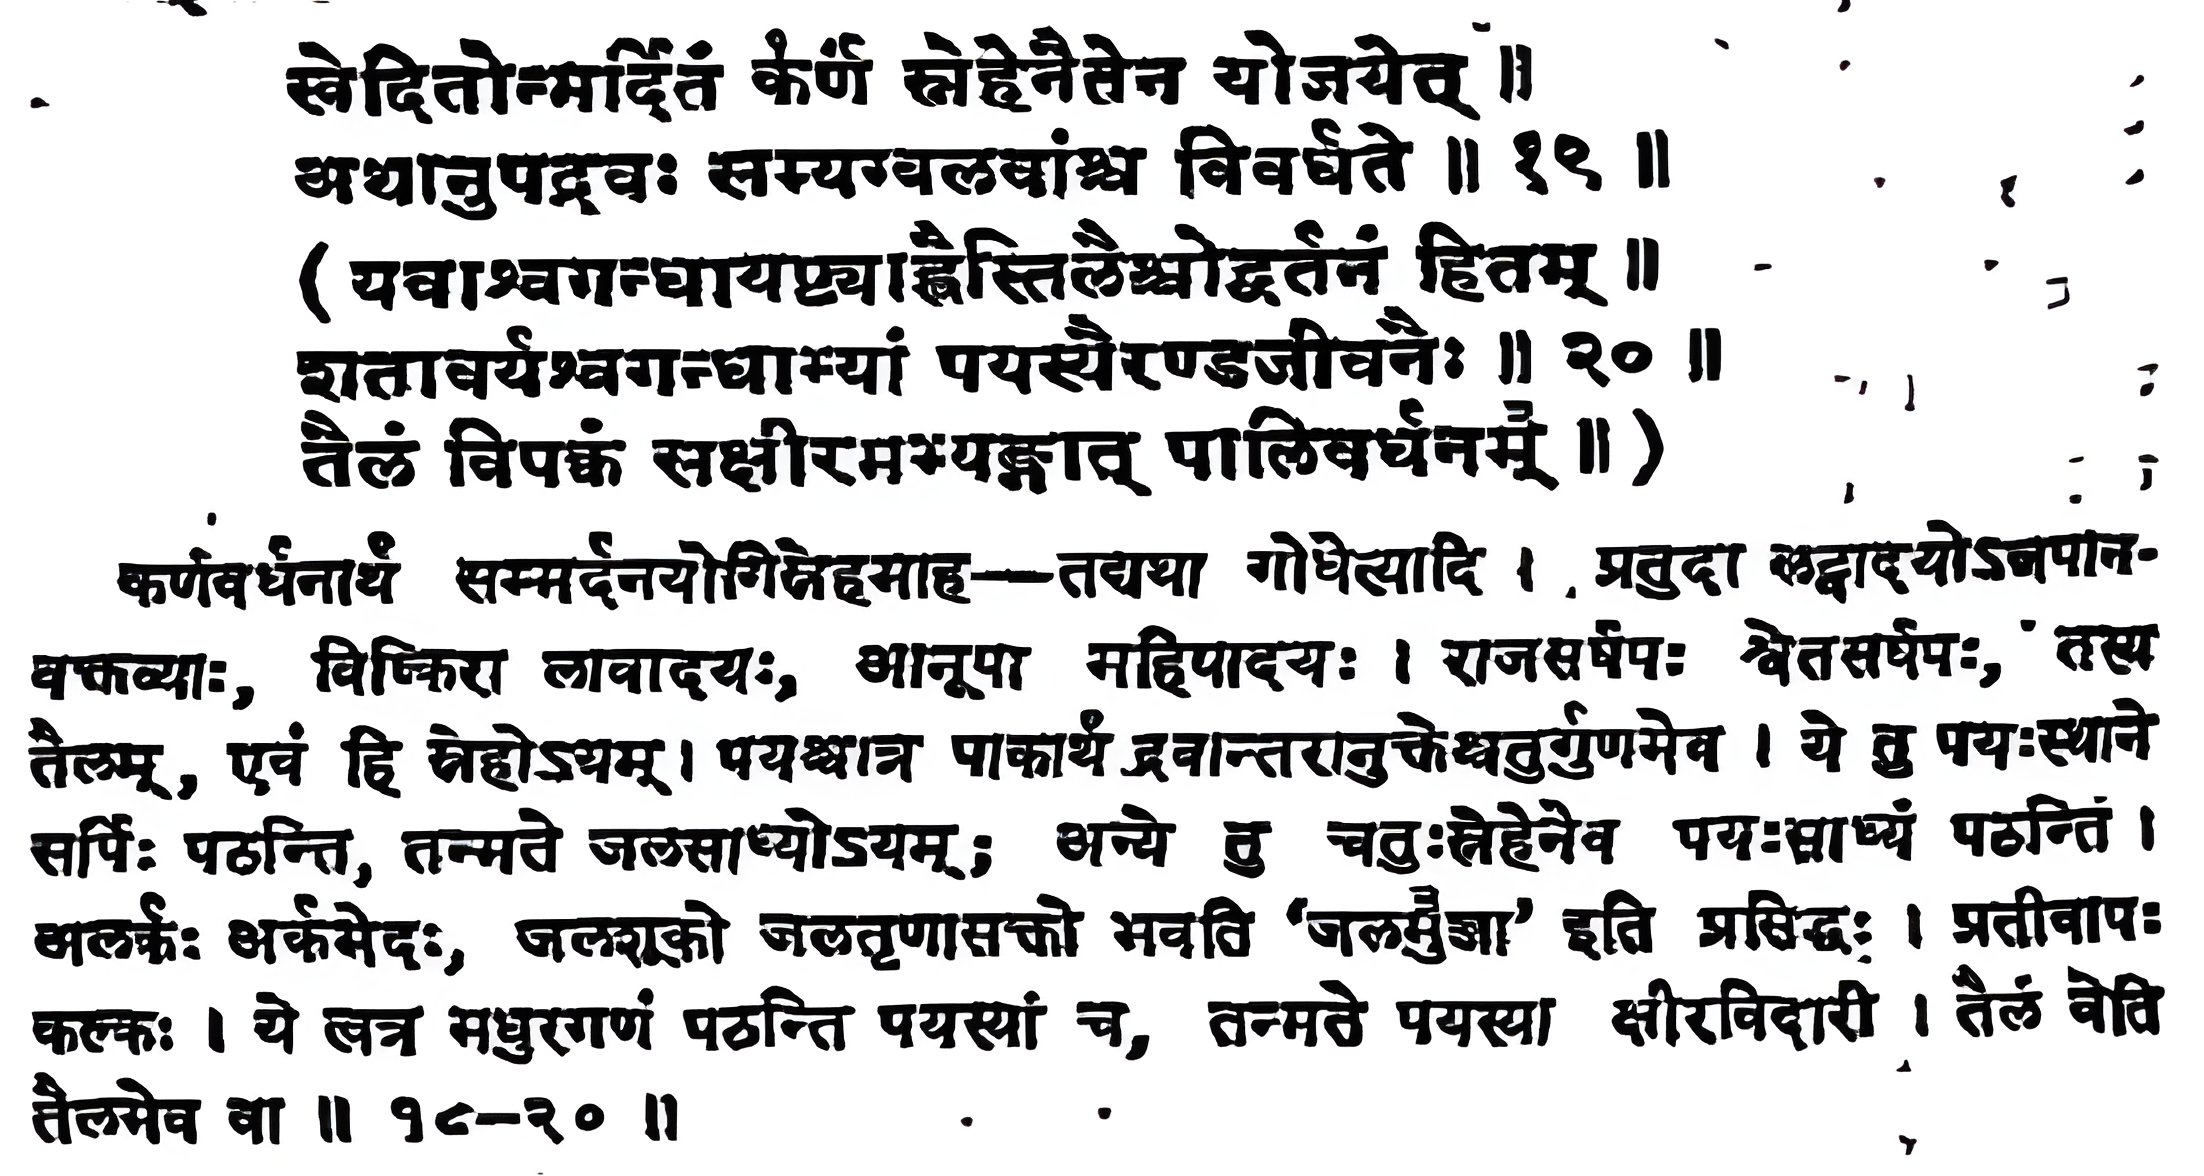
\includegraphics[draft=false,width=.58\textwidth]{media/yavasva-cakra-upscaled}\
    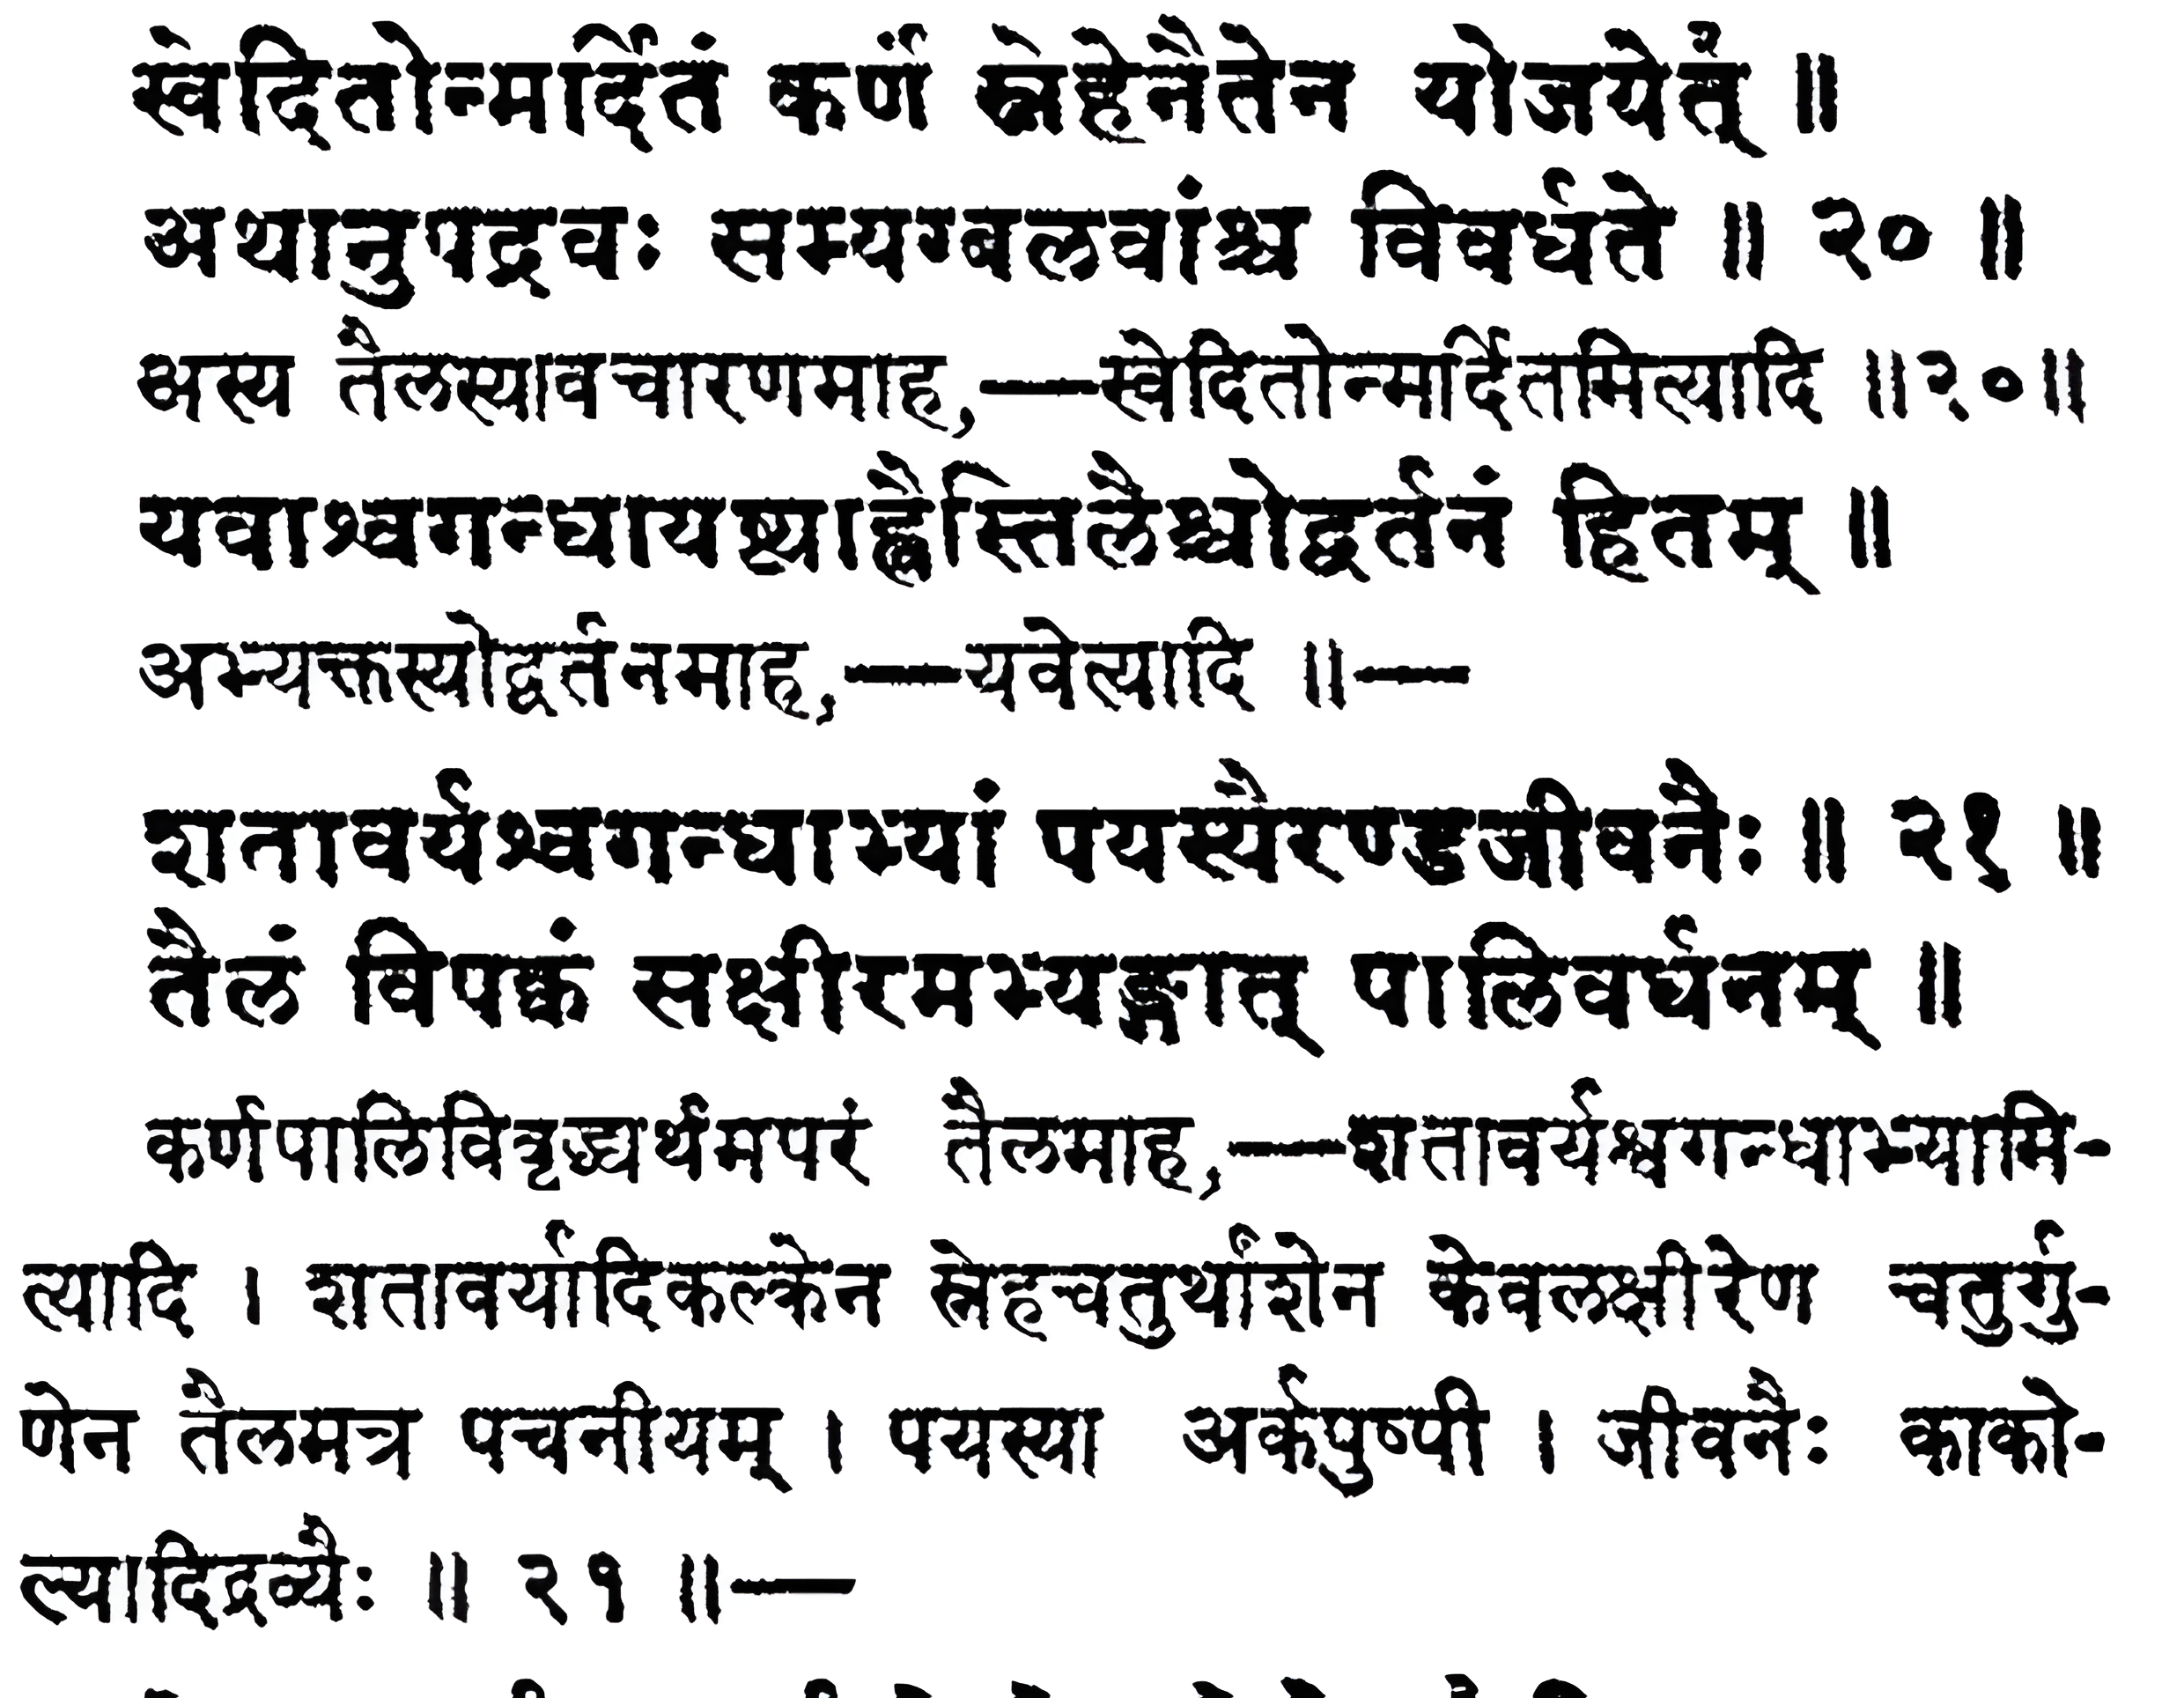
\includegraphics[draft=false,width=.41\textwidth]{media/yavasva-dalhana-upscaled}
    \caption{The text as it appears in Cakrapāṇi (left) and Ḍalhaṇa (right)  
    (\cite[130]{acar-1939}, \cite[79]{vulgate}).}
    \label{fig:yavasva}
\end{figure}
citing keywords that show they all formed part of the main text of the \SS\ that
was before him.\footnote{\Su{1.16.19--23}{79--80}.} However, Cakrapāṇidatta's
    older commentary showed no awareness of the first few verses in this group, SS
    1.16.19--21ab.\footcite[130--131]{acar-1939}  Apparently, they were \emph{not}
    part of the text of the \SS\ as he knew it.  In spite of that, the editors printed
    these verses in their edition of Cakrapāṇidatta's work as if they were indeed part
    of the \SS\ known to him. Incidentally, the editors remarked in a footnote that
    verses 20--21a were not in the Nepalese manuscript that they consulted.  This
    shows that the version of the \SS\ that Cakrapāṇidatta knew is similar to the
    Nepalese version, at least in this particular case.\footcite[130, n.\,2]{acar-1939}

A similar instance occurs in the edition of the \emph{Bhānumatī} at SS 1.16.31, 
where the editors of the 1939 printed edition included a verse in parenthesis that was
commented on by Ḍalhaṇa but not by Cakrapāṇidatta (see 
Fig.\,\ref{fig:nadiyogam}).\footnote{The verse begins 
\dev{nāḍīyogaṃ vinauṣthasya}.  It is printed in the vulgate as 
\Su{1.16.32}{81}, with Ḍalhaṇa's commentary.  It is printed in parentheses as 1.16.31 in the 
edition of the Bhānumatī \citep[133]{acar-1939}.} This verse was almost certainly not in the 
text of the \SS\ known to Cakrapāṇidatta. 
\begin{figure}[t]
    \centering
    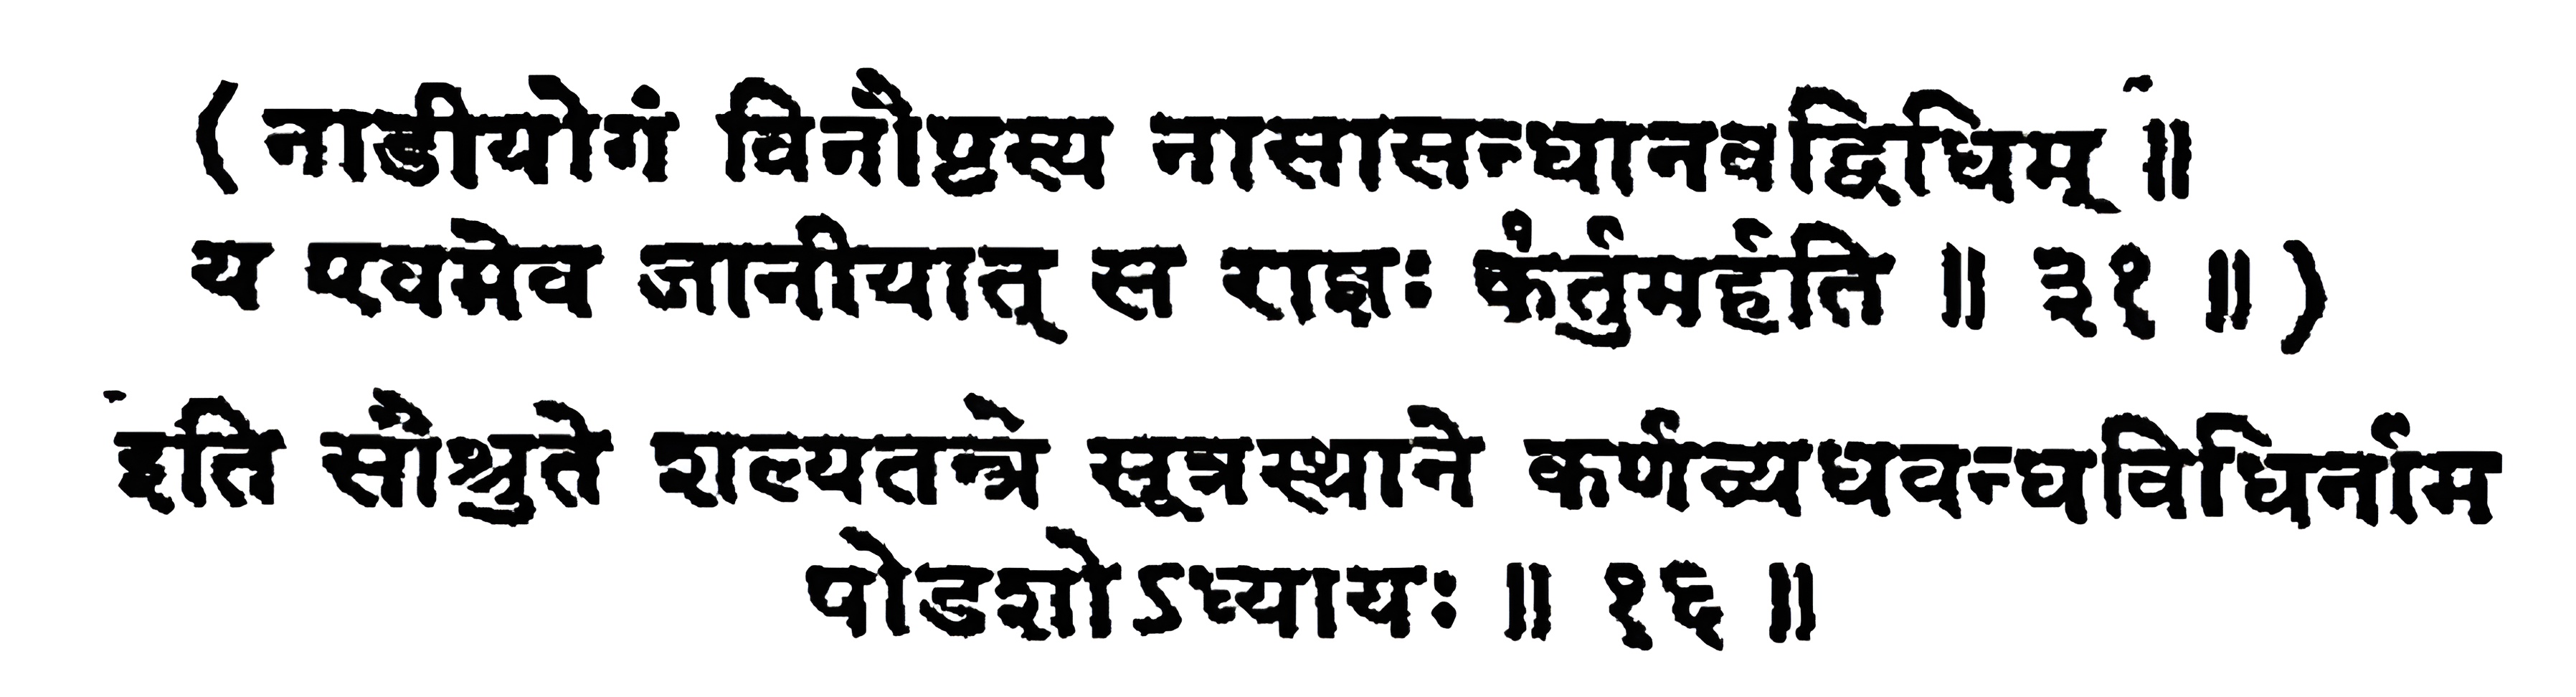
\includegraphics[draft=false,width=.90\linewidth]
    {media/nadiyogam-upscaled}
    \caption{\SS\,1.16.31 in the 1939 printed edition.}
    \label{fig:nadiyogam}
\end{figure}
The manuscript on which the editors' edition of Cakrapāṇidatta's \emph{Bhānumatī}
commentary was mainly based,  \MScite{London BL H. T. Colebrooke 908}, does not
include the root text of the \SS.\footnote{This observation is based on an
    examination of the opening passage \MScite{London BL H. T. Colebrooke 908}. The MS
    is described in \volcite{1.5}[928, \#2647]{egge-1887}. %of MS 1887-1935
    % of the \emph{Bhānumatī},
    % which is transcribed in Eggling 1896: 928.
    %The transcription in this catalogue also shows the commentary without the
    % root
    % text.
    The section “The 1939 Edition,” on p.\,\pageref{1939edition} below, describes
    the sources that the editors used for that edition.}  Therefore, it requires a
    careful reading of the commentary itself to reverse-engineer, as it were, what
    its author, Cakrapāṇidatta, was seeing in the manuscripts of the \SS\ that he
    had before him in the eleventh century. But there is no evidence that they
    included the verses SS 1.16.19–-21ab and 31 that are printed in the
    \cite{acar-1939} edition as if they were present to Cakrapāṇidatta.

% Ḍalhaṇa 1.16.11–14
%The version of 1.16.11–14 known to Ḍalhaṇa \citep[78]{vulgate} has four verses (\emph{śloka}) at this point that are not in the Nepalese manuscripts. The additional verses iterate the types of joins required for ear flaps that are missing, elongated, thick, wide, etc. All four verses were probably absent in the version of the \emph{Suśrutasaṃhitā} known to Cakrapāṇidatta. He cites the verses separately in his commentary, the \emph{Bhānumatī} \citep[128–129]{acar-1939}, introducing each one as 'some people read' (\emph{ke cit paṭhanti}). However,  in Trikamajī Ācārya's edition of the \emph{Sūtrasthāna} of the \emph{Bhānumatī}, the root text is largely identical to the one commented on by Ḍalhaṇa (\cite{vulgate}), even in instances like this where Cakrapāṇidatta's commentary indicates that he was reading a different version of the \emph{Suśrutasaṃhitā}

% Ḍalhaṇa 1.16.19–20 
%Cakrapāṇidatta \citep[131]{acar-1939} does not comment on these verses, nor verse 15 of the Nepalese version, and so the version of the \emph{Suśrutasaṃhitā} known to him may not have included them.

% Ḍalhaṇa 1.16.32
 %Cakrapāṇidatta \citep[133]{acar-1939} does not comment on this additional verse, which suggests that either he did not know of it or was not inclined to accept it.
 
% Both commentators were aware of a version of the \SS\ that was similar to the Nepalese version % See blog.
\section{Cakrapāṇidatta and the Nepalese version}

We have already seen one case where Cakrapāṇidatta's version of the \SS\ was more
similar to the older Nepalese version than to the later version of Ḍalhaṇa.  There
is more evidence for this.  For example, SS 1.16.5 of the Nepalese version begins
with the compound \dev{doṣasamudayāt}; Cakrapāṇidatta began his comment on this
passage by glossing this very expression. By contrast, Ḍalhaṇa's version inserted
two compounds, \dev{kliṣṭajihmāpraśastasūcīvyadhāt} and \dev{gāḍhataravartitvāt},
before this.\footnote{\Su{1.16.6}{77}.} It appears that Cakrapāṇidatta was not
    aware of the compounds that Ḍalhaṇa saw in his later version, but was indeed
    reading a text similar to the Nepalese version.\footnote{1.16.5
        \citep[126–127]{acar-1939}.}
        
If one looks beyond SS 1.16, there are further instances where the Nepalese version and
the root text as read by Cakrapāṇidatta have the same reading, but Ḍalhaṇa
mentioned it as an alternative that is, “read by others.” For example, the Nepalese
version of SS 1.1.22 begins \dev{tatrāsmiñchāstre\ldots}, which is also
the reading commented on by Cakrapāṇidatta.\footnote{1.1.20 (\emph{sic})
    \citep[17]{acar-1939}.} However, Ḍalhaṇa commented on \dev{asmiñchāstre} and
    stated that “others read \dev{tatrāsmiñchāstre}”.\footnote{\Su{1.1.22}{5}.}
        %Also, in his commentary
        % on SS 1.1.8.1,
        %Ḍalhaṇa notes the variant reading \dev{ṣaṣṭyā vidhānaiḥ}, which is not in his
        % root
        %text but evidently was in Cakrapāṇidatta's.\footnote{See \Su{1.1.8.1}{5} and
        %SS 1.1.6 \citep[11]{acar-1939} respectively.}
        
Another example is the reading of \dev{ṣaṣṭyā vidhānaiḥ} in Ḍalhaṇa's commentary
on SS 1.1.8.1 that is not in his main text but that he ascribes to “some
others”.\footnote{1.1.8.1 \citep[3]{vulgate}.} This reading is likely to be derived  from 
the 
expression \dev{ṣaṣṭyābhidhānaiḥ} in the main text of the Nepalese version, and to 
have been rewritten before Ḍalhaṇa's time because it was hard to 
understand.\footnote{See the discussion by \citet[4--5]{birc-2021a}.}

% Ḍalhaṇa was aware of the reading in the Nepalese version because he notes in his commentary on 1.16.6 \citep[77]{vulgate} that some read 'because of the accummulation of humours' rather than 'because of piercing with a painful, crooked and unrecommended needle or because of a wick that is too thick.' 

\section{Differences between the Nepalese and later versions of \SS~1.16}

% The structural differences between the Nepalese and subsequent versions has been 
%discussed by \citet[27–44]{kleb-2021b}, which include the frame story,\footnote{On this 
%topic, also see the more recent \citet{birc-2021}.} the name of the first book 
%(\emph{Ślokasthāna}), the structuring of the text according to chapter and section 
%colophons, 
%and an additional passage in the \emph{Kalpasthāna}. \citet[44–55]{kleb-2021b} also 
%makes 
%general observations on distinct features of the Nepalese version's content and looks 
%specifically at lists of skin lesions arising from urinary disease and vital energies. And in an 
%effort to demonstrate the possibility of greater coherence in the Nepalese version, 
%\citet[101–104]{hari-2011} has compared its classification of snakes with Ḍalhaṇa's 
%version. 

% On the whole, these observations indicate that [...synopsis of general conclusions here, Andrey?...]
%% 1.16 is missing yathovāca bhagavān dhanvantariḥ|

Several differences between the text of the \SS\ as reconstructed on the basis of
the Nepalese MSS and as found in its multiple contemporary printed editions have
already been pointed out in previous publications.  For example,
\citeauthor{kleb-2021b} listed differences in the chapter sequences as they
affect the overall organization and structuring of themes and elements of the
text.\footcite[27\,f.]{kleb-2021b} Others have explored variations in the frame
story of the work as a whole.\footcites{wuja-2013} [28-32]{kleb-2021b}
{birc-2021} [2-4]{birc-2021a} \citeauthor{kleb-2021b} discussed the
interchangeable use of two titles for the first book of the text, namely
“\emph{Ślokasthāna}” and “\emph{Sūtrasthāna}.” He also discussed another feature
of the Nepalese version, namely the additional colophons found at
the end of each book and also at the end of each decade of chapters of the
work.\footcite[32--44]{kleb-2021b}

\subsection{The greater internal coherence of the Nepalese version}

In an exemplary investigation of textual variants in the Nepalese version,
Harimoto studied the classification of snakes in SS 5.4 and revealed that the
Nepalese version preserves a text that is internally more consistent and coherent
than the versions of the \SS\ found in different printed
sources.\footcite[101–104]{hari-2011}

Klebanov contributed some further general remarks and examples of substantive
differences between the Nepalese and vulgate versions, and provided two more case
studies.\footcite[44--55]{kleb-2021b} The first dealt with the list of skin
lesions associated with urinary disease.\footnote{\dev{pramehapiṭakā} in the
    Nepalese spelling.}  Their signs and pathogenesis are described in the
    \emph{Nidānasthāna} and their treatment in the \emph{Cikitsāsthāna}.\footnote{\SS\
        \Su{2.6}{289--294} and \Su{4.12}{454--455} respectively.} This list of skin
        lesions exemplifies a case where the Nepalese version of the \SS\ is internally
        more coherent than that commented on by Ḍalhaṇa. The incoherence of Ḍalhaṇa's
        version was already identified by an earlier commentator, Gayadāsa
        (fl.\,ca.\,1000), who proposed a textual conjecture that corresponds to the
        reading of the Nepalese version.\footnote{\MScite{Kathmandu KL 699} was copied a
            century or more before Gayadāsa's time, so its version cannot have been 
            influenced
            by Gayadāsa's innovations or suggestions.  The reverse is more likely, although 
            we
            are still uncertain of whether Gayadāsa was aware of the Nepalese version. Being
            from Bengal, it is not unlikely that he knew it.}

The second case study by \citeauthor{kleb-2021b} focussed on the variation in the
list of bodily winds (\dev{prāṇa}) in SS 3.4.\footcite{kleb-2021b}  This
discussion  too relied upon Gayadāsa's learned remarks. He commented on a version
of the \SS\ corresponding to the Nepalese version and reported an alternative
reading and its interpretation preferred by another ancient commentator, Jejjaṭa
(fl.\,ca.\,650 -- c.\,750). It is Jejjaṭa's reading that is known to modern
readers of the \SS\ from the vulgate version of the text.

%The present study also provides a telling example of interpolation, at line 60. 
%This is a rare case in which we have a fairly good idea of where the inserted text
%came from, namely the medical theory associated with the 
%\emph{Carakasaṃhitā}.\q{Give the Ca. reference.}

As the present study demonstrates, many features pertaining to the actual
content of the Nepalese version continue to come to light as we proceed with our
study of the manuscripts.  On the whole, these observations indicate that many
features of the Nepalese version of the \SS\ are likely to go back to an early
state of the work that was common to other versions of the compendium. However,
there are also textual features, such as the text-structuring colophons concluding every
tenth chapter, are likely to have occurred within a local Nepalese transmission of
the text and it is unlikely that they will be attested in MSS from other regions,
when a study of those is done. When evaluating the Nepalese readings historically,
it is necessary to keep in mind that there is plentiful evidence that Ḍalhaṇa's
version of the text also included extremely early readings and variants,
suggesting that some of the readings accepted by Ḍalhaṇa were ancient, if not
original.  Each case has to be weighed, and we are not yet in a position to make 
definitive jugements about the early divergence of textual recensions. 

The detailed comparison that follows of 1.16 of the Nepalese version with
Ḍalhaṇa's \emph{Nibandhasaṅgraha} unfolded as the chapter was edited. The
differences appear to emanate largely from attempts in Ḍalhaṇa's version to
standardise, simplify or clarify the language that appears in the Nepalese
version, to add and redact information, and introduce changes to recipes and
therapies. Examples from 1.16 have been provided to demonstrate these general
observations which, we expect, will be supported by a larger survey of the text.

\subsection{Transpositions}


Figure \ref{fig:chapters} reveals the extent to which 1.16 of the Nepalese version
was redacted to create the one known by Ḍalhaṇa. In this particular case,
twenty-seven verses have been added in the vulgate.  Eight of these verses
(11--14, 21--22ab, 23cd--24, 32) are well integrated with the existing material in
so far as they reiterate and elaborate on the content of passages in the Nepalese
version. A block of nineteen verses (26.1--19) at the end of this chapter in
Ācārya's edition of the \emph{Nibandhasaṅgraha} (\cite[80]{vulgate}) was known by
Ḍalhaṇa. These verses cover additional diseases of the ear lobes, with their
treatment and complications. Although Ḍalhaṇa conceded that some predecessors read
them in this chapter, he concludes that they were not composed by sages and,
therefore, should not be read. Ācārya probably included these verses because they
were in his manuscripts, but Ḍalhaṇa's comments prompted him to place them in
parentheses.\footnote{Ācārya (\cite[80]{vulgate}) did not state that these verses
    were absent in some or all of his manuscripts, which he usually did in a footnote
    if this was the case. A broader survey of manuscripts would be helpful for
    establishing whether these verses were part of the transmission of the \SS\ in
    other parts of India. For example, they are present in \MScite{Hyderabad Osmania
    137-3(b)}.}  Be this as it may, this large block of verses is not present in the
    Nepalese version.
\begin{figure}[t]
\centering
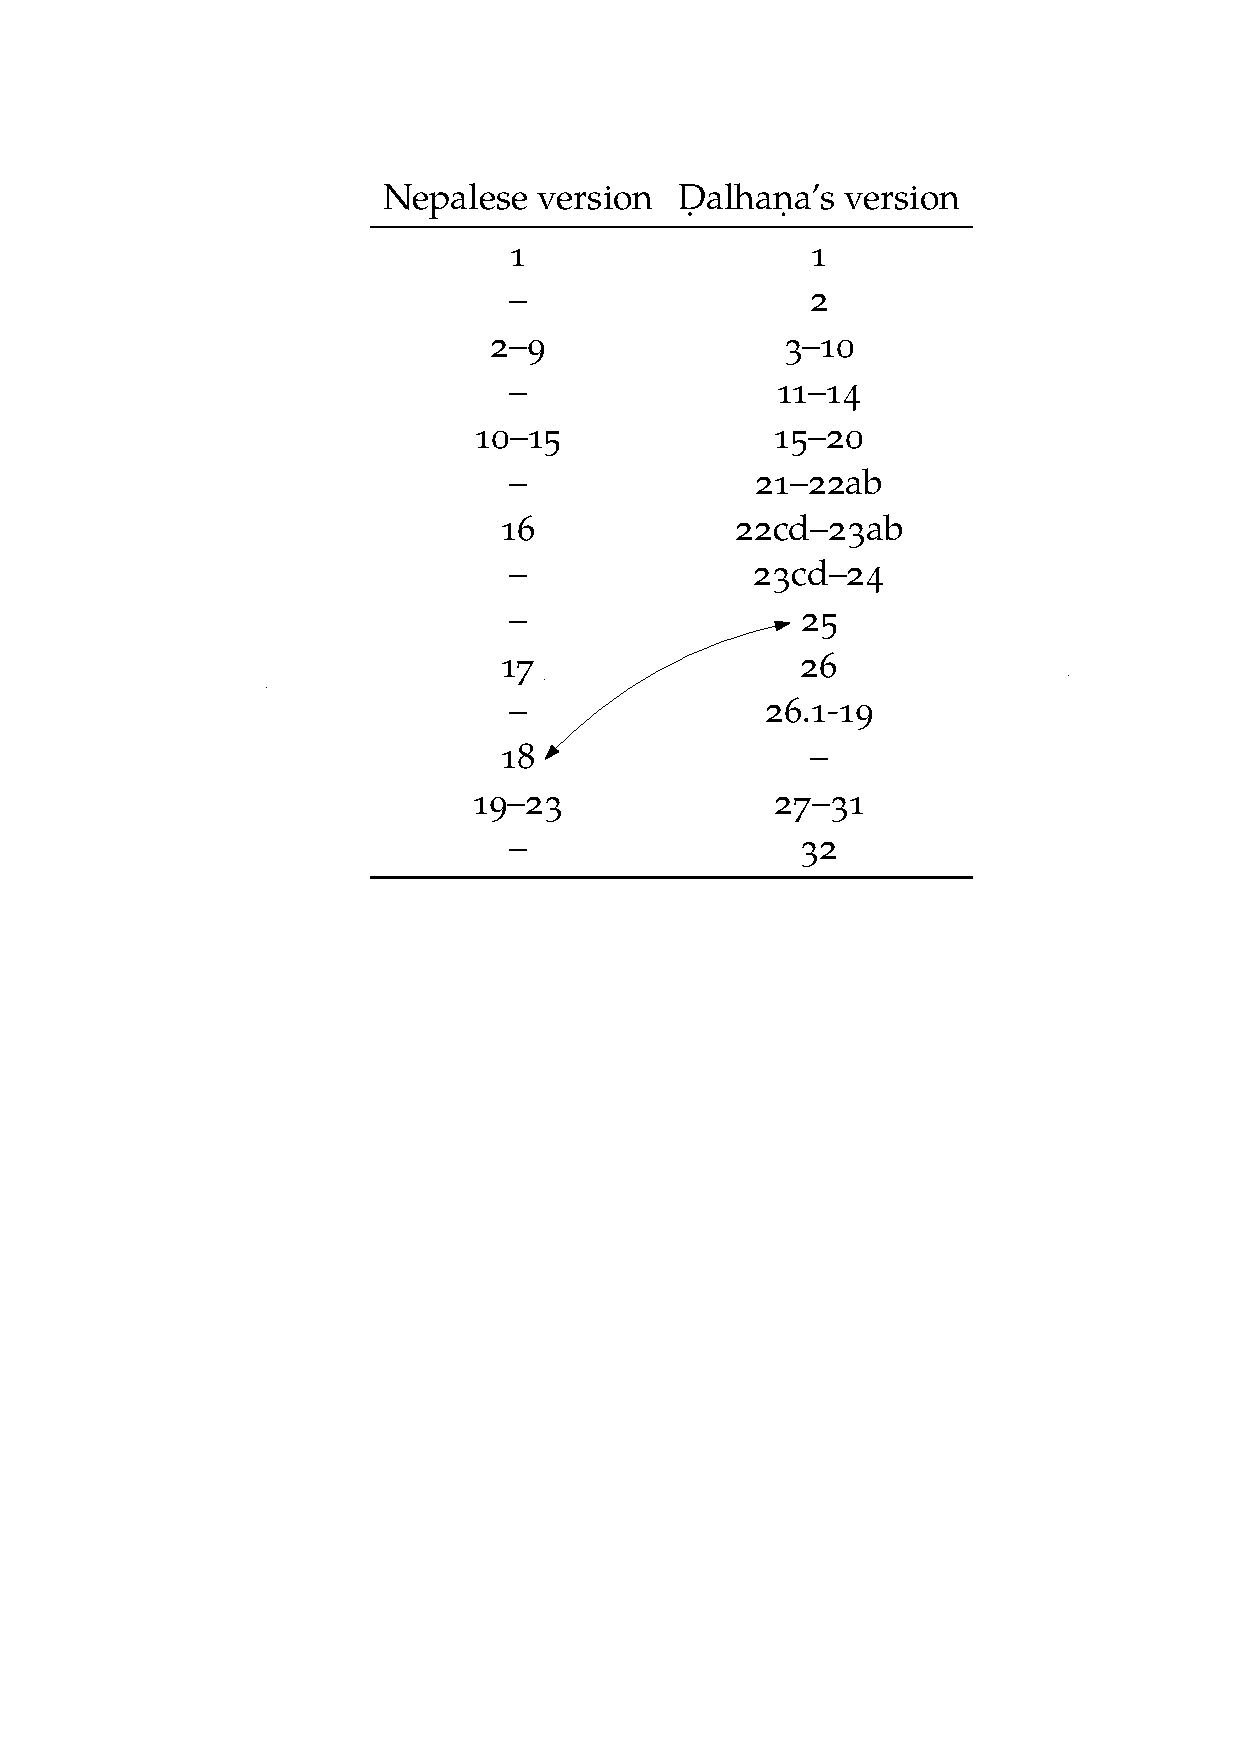
\includegraphics[draft=false,width=.75\textwidth]{media/table-of-versions.pdf}
\caption{A Comparison of verses in 1.16 of the Nepalese and Ḍalhaṇa's versions.}
\label{fig:chapters}
\end{figure}

One can also see in Figure \ref{fig:chapters} that verses 17 and 18 of the
Nepalese version were transposed in the redaction of Ḍalhaṇa's version, where
they are numbered 26 and 25 respectively. Although this only occurs once in 1.16,
such transposing of verses and even their hemistiches is common in the
redaction of other chapters of the \SS.

Apart from the addition of verses, the redacting of the version known to Ḍalhaṇa
involved many small, yet sometimes significant, changes that are described
below.\footnote{The present study focusses on the commentary of Ḍalhaṇa, but many
    of the same investigations could be made with regard to the surviving parts of the
    other early commentaries. See the discussion below, p.\,\pageref{ref:dalhana}.}

\subsection{Changing Spelling, Sandhi and Syntax}


Later commentators like Ḍalhaṇa often made efforts to standardise, simplify or
improve the language of the Nepalese version. Such changes include the
standardising of spelling,\footnote{For example, \dev{pattāṅga} (SS 1.16.21) →
    \dev{pataṅga} (1.16.29, \cite[81]{vulgate}). For more information on this, see
    footnote \ref{pattanga} to the translation.} sandhi,\footnote{For example,
        \dev{°hastena ṛju} (SS 1.16.2) → \dev{°hastena rju} (1.16.3, \cite[76]{vulgate}).}
        and verbal forms,\footnote{For example, \dev{unnāmayitvā} (SS 1.16.21) →
            \dev{prānnamya} (1.16.29, \cite[81]{vulgate}); \dev{avacūrṇayīta} (SS 1.16.21) 
            →
            \dev{upaharet} (1.16.29, \cite[81]{vulgate}).} as well as interventions to
            simplify and clarify syntax.\footnote{For example, 
            \dev{śoṇitabahutvanivedanāyāṃ
                cānyadeśaviddhamiti jānīyāt | nirupadravatā taddeśaviddhaliṅgam/} 
                (SS 1.16.3) →
                \dev{śoṇitabahutvena vedanayā cānyadeśaviddhamiti jānīyāt/ nirupadravatayā
                taddeśaviddham iti/} (1.16.4, \cite[76]{vulgate}); 
                \dev{āmatailapariṣekeṇopacaret}
                (SS 1.16.6) → \dev{āmatailena pariṣecayet} (1.16.7, \cite[77]{vulgate});
                \dev{suparigṛhītaṃ} (SS 1.16.10) → \dev{suparigṛhītaṃ ca kṛtvā} (1.16.15,
                \cite[78]{vulgate}); \dev{anena} (SS 1.16.15) → \dev{snehenaitena} (1.16.20,
                \cite[79]{vulgate}).} These efforts often involved splitting
                compounds.\footnote{For example, \dev{yadṛcchāviddhāyāṃ sirāyām} 
                (SS 1.16.4) →
                    \dev{yadṛcchayā viddhāsu sirāsu} (1.16.5, \cite[76]{vulgate});
                    \dev{dhānyāmlakapālacūrṇaṃ} (SS 1.16.10) → \dev{dhānyāmlaṃ 
                    kapālacūrṇaṃ} (1.16.20,
                    \cite[78]{vulgate}).} In some instances, these changes improved the
                    grammar,\footnote{For example, \dev{surāmaṇḍakṣīram} (SS 1.16.10) →
                        \dev{surāmaṇḍaṃ kṣīram} (1.16.15, \cite[78]{vulgate}).} or altered the
                        meaning.\footnote{For example, \dev{kṣīṇālpamāṃsaḥ} (SS 1.16.12) →
                            \dev{kṣīṇo'lpamāṃsaḥ} (1.16.17, \cite[79]{vulgate}).} However, some 
                            prefixes of
                            verbal forms,\footnote{For example, \dev{samvarddhitaḥ} (SS 1.16.8) 
                            →
                                \dev{vivarddhitaḥ} (1.16.9, \cite[77]{vulgate}); \dev{niveśya} 
                                (SS 1.16.10) →
                                \dev{sanniveśya} (1.16.15, \cite[78]{vulgate}); \dev{avabadhya} 
                                (SS 1.16.10) →
                                \dev{ca baddhvā} (1.16.15, \cite[78]{vulgate}).} case 
                                endings,\footnote{For
                                    example, \dev{māse} (SS 1.16.2) → \dev{māsi} (1.16.3, 
                                    \cite[76]{vulgate}).} and
                                    indeclinables were changed for less apparent 
                                    reasons.\footnote{For example,
                                        \dev{api} (SS 1.16.13) → \dev{vā} (1.16.18, \cite[79]{vulgate}); 
                                        \dev{ca}
                                        (SS 1.16.16) → \dev{tu} (1.16.23, \cite[79]{vulgate}); \dev{tu} 
                                        (SS 1.16.18) →
                                        \dev{ca} (1.16.25, \cite[80]{vulgate}).} There is also a 
                                        tendency to replace
                                        uncommon words with generic ones,\footnote{For example, 
                                        \dev{mrakṣayet}
                                            (SS 1.16.15) → \dev{yojayet} (1.16.20, \cite[79]{vulgate}); 
                                            \dev{nahyet}
                                            (SS 1.16.21) → \dev{baddhvā} (1.16.29, \cite[81]{vulgate}).} 
                                            add
                                            indeclinables,\footnote{For example, [absent] (SS 1.16.6) → 
                                            \dev{ca} (1.16.7,
                                                \cite[77]{vulgate}); [absent] (SS 1.16.10) → \dev{tatra} 
                                                (1.16.15,
                                                \cite[78]{vulgate}); [absent] (SS 1.16.12) → \dev{api} 
                                                (1.16.17,
                                                \cite[79]{vulgate}).} omit the verb “to be” at the end of 
                                                sentences,\footnote{The
                                                    words \dev{bhavati} or \dev{bhavanti} are omitted four 
                                                    times in Ḍalhaṇa's version
                                                    (1.16.10 (twice), 1.16.17 and 1.16.18 \citep[77, 
                                                    79]{vulgate}).}and introduce
                                                    verses after a prose passage with the phrase 
                                                    \dev{bhavati cātra}.\footnote{For
                                                        example, [absent] (SS 1.16.11) → \dev{bhavati cātra} 
                                                        (1.16.16,
                                                        \cite[79]{vulgate}).}

% Spelling
% 9. nemī → nemi
% 9. yaṣṭī → yaṣṭi
% 9. kākauṣṭhaḥ → kākauṣṭhakaḥ
% 21. pattāṅga → pataṅga *

%Sandhi
% 2 °hastena ṛju  →  °hastena rju (standardise)*

% Standardising and Simplifying Syntax
% 3.  śoṇitabahutvanivedanāyāṃ cānyadeśaviddham iti jānīyāt | nirupadravatā 
%taddeśaviddhaliṅgam// → śoṇitabahutvena vedanayā cānyadeśaviddham iti jānīyāt// 
%nirupadravatayā taddeśaviddham iti//*
% 6 āmatailapariṣekeṇopacaret → āmatailena pariṣecayet*

% Clarifying syntax
%15 anena → snehenaitena*

% Splitting compounds
% 4. yadṛcchāviddhāyāṃ	sirāyām	 → 	yadṛcchayā viddhāsu	sirāsu (clarifies syntax)*
% 10. surāmaṇḍakṣīram → surāmaṇḍaṃ kṣīram (improves grammar)*
% 10. dhānyāmlakapālacūrṇañ → dhānyāmlaṃ kapālacūrṇañ*
% 12. kṣīṇālpamāṃsaḥ → kṣīṇo 'lpamāṃsaḥ (changes the meaning)*

% Changing verbs and gerunds
% 2. vyadhayet → vidhyete (perhaps, picking up on karnau)
% 6. kurvīta → dadyāt (middle to active) 
% 7. muñcet → kuryāt
% 9. bandhyā bhavanti → sādhyāḥ
% 10. suparigṛhītaṃ → suparigṛhītaṃ ca kṛtvā ( attempt to improve syntax)*
% 10. upapādya → upadhārya
% 10. sandarśya → sandadhyāt | tato (attempt to simplify the sentence)
% 13. chidyeta → chidyate (opt to pres)
% 15. mrakṣayet → yojayet * (replacing less common words with generic ones)
% 21. nahyet → baddhvā*
% 21. unnāmayitvā → prānnamya (standardise)*
%21 avacūrṇayīta → avacūrṇayet (standardise)*

% Omitting bhavati
% Happens a few times; e.g., 1.16.9 (twice), 1.16.12, 1.16.13

% Changing Prefixes
% 8. samvarddhitaḥ → vivarddhitaḥ*
% 10. niveśya → sanniveśya*
% 10. avabadhya → ca baddhvā*
% 15. marditaṃ → unmarditaṃ*
% 21. unnāmayitvā → prānnamya *

% Changing case endings
% 2. māse → māsi (shift from māsa to mās. Can't see a reason)
% 3. śoṇitabahutvanivedanāyāṃ →  śoṇitabahutvena vedanayā (splitting compounds, but locative of circumstance or condition changed to instrumental of reason. latter is clearer, but not much in it)
% 19. viśleṣitāyām atha nāsikāyāṃ → °tāyās tv nāsikāyāḥ

% changing indeclinables
%13 anyathā → ato 'nyathā
% 13 api → vā*
% 15 tataḥ → ataḥ
% 16 ca → tu*
% 18 tu → ca*
% 19 atha → tu
% 23 vai → syāt

% Adding indeclinables
% 10 [absent] → tatra
% 6 [absent] → ca
% 9 [absent] → tu
% 10 [absent] → ca
% 12 [absent] → api
% 14 [absent] → vā

% Omitting indeclinables
% 9 tatra → [absent]
% 9 ca → [absent]

%Adding bhavati cātra before verses.

% Not sure
% 2
% kṛtamaṅgalaṃ svastivācanan → kṛtamaṅgalasvastivācanan (the latter makes better sense, but could have been original, in my opinion, or an attempt to better integrate a gloss that had become part of the text.)
% abhisāntvayamānaḥ → abhisāntvayan (shift from Pres Pass Part to Pres Act Part) % It seems only the latter is correct in the given context. So, it could be just an error in the NV. Emend or Change translation!!! 
% % 10. agropaharaṇīyāt appears to be an error in the NV that needs to be emended.

\subsection{Technical Terms}

There is evidence of standardising and altering technical terminology in versions
of the \SS\ subsequent the Nepalese one. Two examples of this in \SS\,1.16 are the
terms for “joins” (\dev{bandha})\sse{bandha}{joins} and “a slice of flesh”
(\dev{vadhra})\sse{vadhra}{a slice of flesh}. The Nepalese version uses three
terms for “joining” splits in the ear flaps and the flesh of nose (\dev{bandha,
    sandhāna, sandhi})\sse{bandha, sandhāna, sandhi}{joining}. Redactors of 
    subsequent
versions appear to have tried to standardise this terminology by replacing
\dev{sandhāna} and \dev{sandhi} with \dev{bandha} in prose passages.\footnote{For
    example, \dev{pañcadaśasandhānākṛtayaḥ} (SS 1.16.9) → 
    \dev{pañcadaśabandhākṛtayaḥ}
    (see \Su{1.16.10}{77}); \dev{daśakarṇasandhivikalpāḥ} (SS 1.16.9) →
    \dev{karṇabandhavikalpāḥ} (see \Su{1.16.10}{77})} However, the use of the term
    \dev{sandhāna} was retained in verses, perhaps because of the metrical challenges
    of making such a change or perhaps because the verses 
    had greater traditional authority. Also, the names of joins which incorporate 
    \dev{sandhāna}
    and \dev{sandhi} remained the same.\footnote{These names are 
    \dev{nemīsandhānaka},
        \dev{kapāṭasandhika}, and \dev{ardhakapāṭasandhika} in SS 1.16.9 (cf.\
        \Su{1.16.10}{77}).}

The Nepalese version contains the rather obscure term \dev{vadhra} for the slice
of flesh that a surgeon cuts from the cheek in order to construct a new
nose.\footnote{SS 1.16.20 and 23.} Modern dictionaries define \dev{vadhra} as a
    leathern strap or a slice of bacon,\footcites[1385]{apte-prac}[917]{moni-sans} the
    latter of which is more indicative of its meaning in the Nepalese version. This
    word was written out of subsequent versions,\footnote{\dev{vadhram} (SS 1.16.20) →
        \dev{baddham} (SS 1.16.28, \cite[81]{vulgate}) and \dev{tadvadhraśeṣaṃ}
        (SS 1.16.23) → \dev{tadardhaśeṣaṃ} (SS 1.16.31, \cite[81]{vulgate}).} and it was
        not mentioned as an alternative reading by either Cakrapāṇidatta or Ḍalhaṇa, which
        suggests that its use and meaning may not have been known to them. However,
        \dev{vadhra} was used by the author of the \emph{Aṣṭāṅgahṛdayasaṃhitā} in the
        context of rhinoplasty, so it likely to be the correct reading in the Nepalese
        version.\footnote{\Ah{Utt.18.62}{841}. This may suggest some indepencence 
        between
            the text of the \SS\ as transmitted to its direct commentators and as transmitted
            to Vāgbhaṭa. The word \dev{vadhra} is old, occurring, also in the form
            \dev{vardhra}, from the \emph{Atharvaveda} onwards
            \pvolcite{2}[521--522--277]{mayr-1986}.}



% bandha
% 1. athātaḥ karṇavyadhavidhim vyākhyāsyāmaḥ  → athātaḥ karṇavyadhabandhavidhim adhyāyaṃ (prose)
% sandhāna in all version (verse)
% 9. pañcadaśasandhānākṛtayaḥ (SS 1.16.9) → pañcadaśabandhākṛtayaḥ (SS 1.16.10) 
%(sandhāna is reflected in the name nemisandhānaka, which is in all versions) 
% 9. daśakarṇasandhivikalpāḥ → karṇabandhavikalpāḥ (sandhi is in many of the names, bandha is not)
% 10. (twice) bandha in all versions
% 17 karṇabandha in all versions
% 19 & 23. sandhāna accepted in all versions + 32 in DV. (verse)
% 20. sādhubaddham → sādhubandhaiḥ (verse)
%
% vadhra 
% 20 vadhram → baddham 
% 21 susīvitaṃ → susaṃhitaṃ
% 23 tadvadhraśeṣaṃ → tad ardhaśeṣaṃ

\subsection{Augmenting the Text}

Apart from adding whole passages and verses (as seen in Figure \ref{fig:chapters}),
redactors of subsequent versions augmented the text by expanding existing
compounds and inserting new compounds and words. Within the microcosm of 1.16,
adjectives and adverbs were inserted to clarify statements,\footnote{For example,
    \dev{chidre} (\SuComma{1.16.2}{76}) → \dev{chidra ādityakarāvabhāsite}
    (\SuComma{1.16.3}{76}); [absent] (1.16.2) → \dev{śanaiḥ śanaiḥ} (1.16.3); 
    [absent] (SS 1.16.3) → \dev{āśu} (\SuComma{1.16.5}{77}).} and phrases added to
    elaborate on diseases and treatments.\footnote{For example, \dev{dhātryaṅke}
        (SS 1.16.2) → \dev{dhātryaṅke kumāradharāṅke vā} (1.16.3); [absent] (SS 1.16.2) →
        \dev{bālakrīḍanakaiḥ pralobhya} (1.16.3);  [absent] (SS 1.16.3) →
        \dev{picuvartiṃ praveśayet} (1.16.5).} In particular, the characteristics and
        number of symptoms of a disease, as well as their reasons for arising, tend to
        increase in subsequent versions. For example, the Nepalese version (SS 1.16.5)
        said that the wick in a newly pierced ear should be removed because of aggravated
        humours or a culpable piercing whereas the version known to Ḍalhaṇa 
        (\Su{1.16.6}{77}) included two further reasons, namely, because of piercing with
        a painful, crooked and unrecommended needle or because of a wick that is too
        thick. Some of the split ear flaps in Ḍalhaṇa's version have additional
        characteristics,\footnote{For example, \dev{pīṭhopamapālirnirvedhimaḥ}
            (\SuComma{1.16.9}{77}) → \dev{pīṭhopamapālirubhayataḥ kṣīṇaputrikāśrito
            nirvedhimaḥ} (\SuComma{1.16.10}{77}); \dev{itarālpapāliḥ saṃkṣiptaḥ} 
            (SS 1.16.9)
            → \dev{utsannapāliritarālpapāliḥ saṃkṣiptaḥ} (1.16.10); \dev{tanuviṣamapāliḥ}
            (SS 1.16.9) → \dev{tanuviṣamālpapāliḥ} (1.16.10).} and a list of four symptoms
            associated with incurable joins in the Nepalese version (SS 1.16.19) was increased
            to six in Ḍalhaṇa's version (\Su{1.16.10}{77}). Also, models of
            classifying symptoms were introduced in subsequent versions. For example, the
            Nepalese version (SS 1.16.4) lists the symptoms of mistakenly piercing a duct in
            the ear whereas the version known to Ḍalhaṇa (1.16.5, \cite[76–77]{vulgate})
            classifies these symptoms according to three ducts called \dev{kālikā},
            \dev{marmarikā} and \dev{lohitikā}, which results in some repetition of the
            symptoms mentioned.\footnote{In Ḍalhaṇa's version  (\SuComma{1.16.5}{76–77}), 
            the
                symptoms of fever and pain (\dev{jvara}, \dev{vedanā}) are repeated. This 
                repetition
                does not occur in the Nepalese version. It is possible that this classification
                was not in the version of the \SS\ known to Cakrapāṇidatta (1.16.4,
                \cite[126]{acar-1939}) because he mentions that some read classifications of ducts
                at this point in the text and he cites verses from Bhoja on \dev{kālikā},
                \dev{marmarikā} and \dev{lohitikā}, but he does not gloss or comment on the
                passage known to Ḍalhaṇa.}

% Supplementary compounds and phrases for Adding Information
% This is done by expanding compounds, inserting new compounds and adverbs and adding verses and passages.
% 
% 1. karṇavyadhavidhim → karṇavyadhabandhavidhim (foregrounding the term bandha)
% 2
% dhātryaṅke → dhātryaṅke kumāradharāṅke vā (elaborating on treatment)
% upaveśyābhisāntvayamānaḥ → upaveśya bālakrīḍanakaiḥ pralobhyābhisāntvayan (elaborating on treatment)
% chidre → chidra ādityakarāvabhāsite (clarifying technical term)
% [absent] → śanaiḥ śanaiḥ (clarifying treatment)
% [absent] → picuvartiṃ praveśayet (elaborating on treatment)
% 4 
% [absent] →  kālikāmarmarikālohitikāsūpadravā and dividing the adverse affects according 
%to kālikā, marmarikā and lohitikā. Repetition of vedanā and jvara in this process.(discussed 
%in footnote). teṣu yathāsvaṃ pratikurvīt // (adding symptoms, perhaps with a view to 
%managing them more effectively, according to the type of vein pierced).
% 5
% [absent] → kliṣṭajihmāpraśastasūcīvyadhād gāḍhataravartitvād (adding reasons)
% [absent] → yatra saṃrambho vedanā vā bhavati (adding information about the treatment)
%  [absent]  → āśu (clarifies the treatment)
%  [absent] → tāvad yāvat surūḍha iti (until it is well healed - clarifies the treatment)
%9
% pīṭhopamapālir nirvedhimaḥ → pīṭhopamapālir ubhayataḥ kṣīṇaputrikāśrito nirvedhimaḥ (adding characteristics)
% itarālpapāliḥ saṃkṣiptaḥ → utsannapālir itarālpapāliḥ saṃkṣiptaḥ (adding characteristics)
% tanuviṣamapālir → tanuviṣamālpapālir (adding characteristics)
% baddheṣv api dāhapākasrāvaśophayuktā	na siddhim upayānti → tu śophadāharāgapākapiḍakāsrāvayuktā	na siddhim upayānti (adding symptoms)
% 10
% surāmaṇḍodakābhyāṃ → surāmaṇḍoṣṇodakābhyāṃ (adding characteristics of an ingredient)
% 12
% gāḍhapākarāgavān → dāhapākarāgavedanāvān (adding symptoms)

% Additional Verses and Passages (table 1)
% For passages, see subsub on Elaborating on Treatments.
%  [absent] → 16.11–14 (verses)
%  [absent] → 21–22ab, 23cd–24
%  [absent] → 26.1 – 26.19
%  [absent] → 32

\subsection{Transposing Words, Verses and Passages}

A close comparison of the Nepalese version with the vulgate reveals changes in the 
order of words, sentences and verses. Examples of such transpositions occur in SS 1.16. 
In 
most cases, the changes in word order are insignificant and may be result of different 
preferences in syntax or even scribal eye-brain-hand miscommunication.\footnote{For 
example, \dev{aṇusthūla°} (SS 1.16.9) → \dev{sthūlāṇu°} (1.16.10, \cite[77]{vulgate}); 
\dev{tatraite daśakarṇa°} (SS 1.16.9) → \dev{tatra daśaite karṇa°} (1.16.10, 
\cite[77]{vulgate}); \dev{nātigāḍhannātiśithilaṃ sūtreṇāvabadhya} (SS 1.16.9) → 
\dev{sūtreṇānavagāḍhamanatiśithilaṃ ca baddhvā} (1.16.10, \cite[77]{vulgate}); 
\dev{pūrvandakṣiṇaṃ kumārasya vāmaṅkanyāyāḥ | pratanuṃ sūcyā bahalamārayā } 
(SS 1.16.2) → \dev{pratanukaṃ sūcyā bahalamārayā/ pūrvaṃ dakṣiṇaṃ kumārasya 
vāmaṅkanyāyāḥ} (1.16.3, \cite[76]{vulgate}).} However, the transposition of verses and 
passages is usually the result of efforts at redacting the text to add new material. A good 
example of this is the transposition of SS 1.16.17 and SS 1.16.18 in the Nepalese version 
to 
1.16.26 and 1.16.25, respectively, in Ḍalhaṇa's. It seems that this transposition may have 
resulted from the insertion of new verses 1.16.23cd–24 and 1.16.26.1–19 in the latter.

% Words
% 9. aṇusthūla° → sthūlāṇu°
% 9. tatraite daśakarṇa° → tatra daśaite karṇa°
%  10. nātigāḍhan nātiśithilaṃ sūtreṇāvabadhya → sūtreṇānavagāḍhaman atiśithilaṃ ca baddhvā
% Passages
% 2. pūrvan dakṣiṇaṃ kumārasya vāmaṅ kanyāyāḥ | pratanuṃ sūcyā bahalam ārayā // → 
%pratanukaṃ sūcyā bahalam ārayā// pūrvaṃ dakṣiṇaṃ kumārasya vāmaṅ kanyāyāḥ //
% Verses
%17 and 18 → 26 and 25

%
\subsection{Redacting Recipes and Elaborating on Treatments}

Some of the additional text in subsequent versions of the \SS\ introduces new
ingredients in recipes and different procedures in treatments. In many instances,
the new material merely clarifies or elaborates on the original but sometimes it
changes the recipe or treatment significantly.  An example of a suppletion that
clarifies the text of the Nepalese version can be seen in 1.16.3 of Ḍalhaṇa's
version (\cite[76]{vulgate}), which contains a statement that the physician should
insert a wick\label{wick} of cotton after the ear has been pierced.\footnote{For 
example,
    [absent] (SS 1.16.2) → \dev{picuvartiṃ praveśayet} (1.16.3, \cite[76]{vulgate}).}
    This statement anticipates the instructions in the the Nepalese version
    (SS 1.16.5–6) on removing the wick because of aggravated humours and replacing the
    wick with a thicker one every three days. In this case, the additional statement
    of Ḍalhaṇa's version elucidates the role of the wick in the procedure of piercing
    the ear.

A similar clarification occurs in Ḍalhaṇa's version at
\Su{1.16.18}{70},\footnote{Corresponding to SS 1.16.13 in the Nepalese version,
    lines 60--62 of the edition.} which reiterates the cure for an ear tainted by a
    humour that was described earlier in 1.16.7.\footnote{SS 1.16.6 in the Nepalese
        version, lines 16--17 of the edition.} The reiteration is quite apt because it
        follows a passage that outlines the various symptoms of ear disease arising from
        each of the three humours.\footnote{Ḍalhaṇa \Su{1.16.17}{79}, corresponding to
            Nepalese SS 1.16.12, lines 56--59 of the edition.} The author of the Nepalese
            version probably assumed that, after reading SS 1.16.12, the reader would refer
            back to SS 1.16.6 for the cure of an ear affected by a humour. However, in
            Ḍalhaṇa's version, the treatment is reiterated.

In Ḍalhaṇa's version of 1.16, there are two instances in which ingredients were
added to recipes of medicines in the Nepalese version. The first is the recipe of
an ointment that should be applied to a pierced ear that has not healed. In
Ḍalhaṇa's version,  the recipe was rewritten to include sesame
seeds.\footnote{Nepalese version SS 1.16.5 (lines 13--15):
    \dev{yavamadhukamañjiṣṭhāgandharvahastamūlairmadhughṛtapragāḍhairālepayet} 
    which
    become, in Ḍalhaṇa \Su{1.16.7}{77}:
    \dev{madhukairaṇḍamūlamañjiṣṭhāyavatilakalkairmadhughṛtapragāḍhairālepayet}.} 
    A more significant change occurs in another recipe for an admixture of an oil that
    is supposed to be rubbed into a healthy ear to enlarge it. Ḍalhaṇa's version
    of the admixture has five additional ingredients,
    namely, \gls{apāmārga}, \gls{aśvagandhā}, \gls{kṣīraśuklā},
    \gls{madhuravarga}\label{kakolyadi} and \gls{payasyā}.\footnote{Ḍalhaṇa's version 
    \Su{1.16.7}{77}.} %\footnote{The
    %items which exemplify the `sweet' savour \label{kakolyadi}
    % (\dev{madhuravarga})
    % are
    %enumerated at SS 1.42.11.} and \gls{payasyā}. (\dev{payasyā} $\rightarrow$
    %\dev{vidāri}\footnote{Pueraria tuberosa (Willd.) DC. (ADPS 510, IMP 1.792f.,
    % AVS
    %4.391;
    %not Dymock 1.424f. See GJM supplement 444, 451, IMP 1.187, but IMP 3.1719 =
    %Ipmoea
    %mauritiana, Jacq.). }).
    It also has \gls{vidārigandhā} instead of
    \gls{vidārī}.\footnote{Nepalese version SS 1.16.14 (lines 65--66): 
    \dev{arkālarkabalātibalānantāvidārīmadhukajalaśūkaprativāpantailampācayitvā}
which
become, in Ḍalhaṇa \Su{1.16.19}{79}:
    \dev{arkālarkabalātibalānantāpāmārgāśvagandhāvidārigandhākṣīraśuklājalaśūkamadhuravargapayasyāprativāpaṃ
     tailamvā pācayitvā}.}
     
 The general tendency in re-formulating a recipe from the Nepalese version
in later versions of the \SS\ was to preserve most ingredients of the
original and to add new ones.
    
    %\q{Perhaps, Dr Madhu could add
        %a comment on whether these additional ingredients would change the effects of 
        %the
        %treatment in any significant way?}
% % % % % % % begin from Madhu Parameswaran

\section{Comparative therapeutics} 

For at least two reasons, it is interesting to compare the text materials of the
\SS~1.16 with parallel materials found in other texts, including the \CS,  \AS,
and \AHS. The latter two works, both ascribed to Vāgbhaṭa, can safely be dated
to a period after the composition of the \SS\ but before the commentator Ḍalhaṇa,
thus throwing light on a period of development for which witnesses are limited and
also also broadly the period at which the Nepalese version was current. Secondly,
the manner in which Vāgbhaṭa's works incorporate and modify materials from the
\SS\ can help us to understand how recipes and therapies evolved within specific
lines of textual transmission.

The materials presented in \SS~1.16 are parallel to those in two chapters of
the \AS, namely \emph{Uttarasthāna}, chapters 1 and 22, titled
“\emph{bālopacaraṇīya}” and “\emph{karṇarogapratiṣedha},” and \AHS,
\emph{Uttarasthāna} 1 and 18 with the same chapter
names.\footnote{\cite[619--629 and 734--744]{atha-1980} and \cite[777--781
    and 837--841]{kunt-1939}, respectively.}

First, let us return to the comments on the insertion of a wick that were
mentioned above (p.\pageref{wick}).
    %take up the end of
    % passage 2 (line 6)
    % in
    % the edition of the Nepalese
    %version below, corresponding to SS \Su{1.16.3}{76} in Ḍalhaṇa's
    % version.
    %Page 23, % paragraph 1
    The Nepalese version says nothing, while Ḍalhaṇa's version says “one
    should insert a cloth wick” (\dev{picuvartiṃ praveśayet}).  A little
    later, both versions say, “one should remove the
    wick”.\footnote{\dev{tatra varttimapahṛtya} in the Nepalese version
        (line 13), and the less clear \dev{tatra varttimupahṛtya} in Ḍalhaṇa's
        version (\Su{1.16.6}{77}).}  It seems likely that the editor of
        Ḍalhaṇa's version added the initial phrase about inserting the wick
        because it seemed necessary to say that the wick was applied before
        being removed.  The older Nepalese version seems slightly less coherent
        on this point, but is perhaps represents an earlier version of the text
        on the principle of \emph{lectio dificilior potior}. %
        Both the \AS\ and the \AHS\ describe first inserting a thread in the
        pierced earlobe and subsequently replacing it every third
        day.\footnote{\As{6.1.58}{626} and \Ah{6.1.36}{780} respectively.}
            In this repect, they agree  with Ḍalhaṇa’s version.

Secondly, it is interesting to consider again the recipe prescribed to treat
the vitiation of humours in the pierced ear, mentioned above. A slightly
modified recipe is found in the \AS\,\As{6.1.63}{626}, but the same is not
present in \AHS. As pointed out above, Ḍalhaṇa’s version adds a paste of
sesame seeds (\dev{tilakalka}) to the recipe attested by the Nepalese version.
In the parallel version of recipe found in the printed editions of \AS, honey
(\dev{madhu}) is missing, but ghee (\dev{ājya}) is found. However, when
checking the manuscripts of the \AS, one of them reads \dev{ādyaiḥ} instead of
\dev{ājyaiḥ(yavairaṇḍajaṭāyaṣṭīmañjiṣṭhājyaiḥ
    pralepayet)}.\footnote{\MScite{Mumbai, Asiatic Society 162}, catalogue no.\,BD
    263/1--6} Interestingly, the paste of sesame seeds (\dev{tilakalka}) of
    Ḍalhaṇa’s version is not present in the \AS\ and is replaced by \dev{jaṭā},
    which is most probably \gls{jaṭāmāṃsī}. 

Since the  paste of sesame seeds is the main differentiating factor between
the recipe versions attested by the Nepalese version and Ḍalhaṇa’s version, a
general review of the contexts of its use in the major texts may be enlightening.
References for the  paste of sesame seeds are found in the
texts shown in Table~\ref{tilakakalka}.
\begin{table}[h]
    \centering
\begin{tabular}{lr}
    \toprule
\emph{Text}    & \emph{Instances of sesame seed paste} \\
\midrule
\CS    & 6 \\
\SS    & 11 \\
\AS    & 16 \\
\AHS    & 4 \\
    \bottomrule
\end{tabular}
\caption{Sesame seed paste (\dev{tilakalka}) in different texts.}
\label{tilakakalka}
\end{table}
Among them, references with the combination of the  paste of sesame seeds,
ghee and honey are not rare either, with four instances each in \SS\ and \AS\
and two instances in \AHS. A combination of the  paste of sesame seeds, ghee
and honey has also been specifically quoted as a general healing
recipe.\footnote{E.g., \SS\ \Su{1.11.22ab}{49}, \AS\ \As{1.38.21}{249--250}
    and \AHS\ \Ah{1.30.34}{357}.}

Another matter of interest is the combination of ghee and honey. We find many
instances where this unique combination alone or in combination with other drugs
is used in a variety of clinical contexts including those prescribed for the
healing of ulcers or surgical wounds.\footnote{E.g., \AS\ \As{1.37.30}{246} for
    \dev{kṣatakaṇṭha} and \AS\ \As{4.17.22}{517} for healing of the surgical wound in
    \dev{udararoga}.}

This material evidence points to the general trend that medicines in the older
Nepalese version of the \SS\ present a central core recipe, consisting of a
few drugs, that develops with ever-increasing complexity in the more recent
version of Ḍalhaṇa and later authors.

%The general trend over time between the older Nepalese version of the \SS\ to the
%more recent version of Dalhana is an ever-increasing complexity of recipes. This
%is visible, for example, in the addition of new drugs such as \emph{tilakalka},
%the unctuant added specifically to address wind aggravations in a range of
%diseases, to the recipe in the later versions of the text.

% % % % % % % end from Madhu Parameswaran



% 2. [absent] → picuvartiṃ praveśayet (adding a cotton wick after piercing the ear of a boy or girl)
% 5. yavamadhukamañjiṣṭhāgandharvahastamūlair	madhughṛtapragāḍhair ālepayet → madhukairaṇḍamūlamañjiṣṭhāyavatilakalkair madhughṛtapragāḍhair ālepayet (adding the ingredient tila)
% 5  [absent] → tāvad yāvat surūḍha iti [...] vidhānaṃ tu pūrvoktam eva // (until it is well 
%healed [... One should pierce it again by] the method taught earlier- clarifies the 
%treatment)
% 13.  [absent] → āmatailena trirātraṃ pariṣecayet trirātrāc ca picuṃ parivartayet | (extending the treatment)
% 14. arkālarkabalātibalānantāvidārīmadhukajalaśūkaprativāpan tailam pācayitvā →	arkālarkabalātibalānantāpāmārgāśvagandhāvidārigandhākṣīraśuklājalaśūkamadhuravargapayasyāprativāpaṃ tailam vā	pācayitvā (adding ingredients to an oil)
% additional apāmārga, aśvagandhā, kṣīra, 

